\fancychapter{Implementation}
\label{chap:imp}
\textcolor{red}{introdução do capítulo}

\section{DC-DC converter}
\textcolor{red}{introdução do capítulo}

\subsection{Operation principles}
The DC-DC converter chosen for thiis project was a boost converter. This topology uses one switching device, one inductor, one output capacitor and a diode, Figure \ref{fig:boost}. The switching device is used to controol the output voltage by switching on and off at a specified frequency (fsw) and duty cycle (D). The inductor is used to store energy when the switch is on (stage 1) and release it when the switch is off (stage 2), while the output capacitor is used to smooth the output voltage.

\begin{figure}[!h]
    \centering
    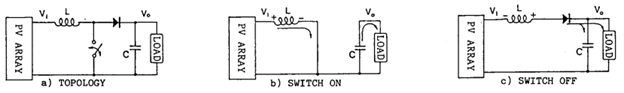
\includegraphics[width=0.9\textwidth]{Images/Implementation/Boost.png}
    \caption{Classic Boost converter topology and stages \cite{Comparison_PV_Converter_Technologies_1989}.}
    \label{fig:boost}
\end{figure}

Analyzing the boost converter speratly on his two stages, it is possible to define the drop  voltage across the inductor (VL), as a function of the input voltage (Vin) and output voltage (Vout) as follows:

\begin{equation}
    V_L = \begin{cases}
    V_{in} & \text{if } t \in [0, D \cdot T] \\
    V_{in} - V_{out} & \text{if } t \in [D \cdot T, T]
  \end{cases}
  \label{eq:vl}
\end{equation}

With equation \ref{eq:vl} and the fact that at stationay state the average voltage across the inductor is zero, it is possible to define the output voltage in function of the input voltage and duty cycle as folows:

\begin{equation}
    V_{Lavg} = \frac{1}{T} (\int_{0}^{DT} V_{in} dt + \int_{DT}^{T} (V_{in} - V_{out}) dt) = 0 \Rightarrow V_{out} = \frac{V_{in}}{1-D}
    \label{eq:duty}
\end{equation}

Equation \ref{eq:duty} is one of the most important equations in boost converter design, as it defines the relationship between the input voltage, output voltage and duty cycle. It is possible to see that as the duty cycle increases, the output voltage also increases, which is the main principle behind boost converters. However this equation is only valid for ideal components since it does not take into acount the parasitic elements of the components, such as the resistance of the inductor and the voltage drop across the diode. In a real boost converter, these parasitic elements will cause a voltage drop and therefore reduce the output voltage.

Lets quickly analyze the influence of the inductor resistance ($R_L$) and the voltage drop across the diode ($V_d$) by changing the equation \ref{eq:vl} to:

\begin{equation}
    V_L = \begin{cases}
    V_{in} & \text{if } t \in [0, D \cdot T] \\
    V_{in} - V_{out} - V_d & \text{if } t \in [D \cdot T, T]
  \end{cases}
  \label{eq:vl2}
\end{equation}

In this case the at stationay state the average voltage across the inductor is $R_L \cdot I_L$ and therefore the output voltage can be defined as:

\begin{equation}
    V_{Lavg} = \frac{1}{T} (\int_{0}^{DT} V_{in} dt + \int_{DT}^{T} (V_{in} - V_{out}) dt) \Leftrightarrow R_L \cdot I_L = \frac{1}{T}[D \cdot  V_{in} + (1-D)\cdot(V_{in} - V_{out} -V_d)] \Leftrightarrow
\end{equation}

\begin{equation}
    \Leftrightarrow V_{out} = \frac{V_{in} - R_L \cdot I_L}{1-D}-V_d
    \label{eq:vout2}
\end{equation}

Equation \ref{eq:vout2} swhows the 2 mains causes of losses in a boost converter. The main cause is the voltage drop across the diode, which causes a significat reduction in the output voltage (usaly 0.3~V to 0.7~V). This can be solved by using a synchronuos boost converter, which replaces the diode with a transistor. In synchronous boost conveters the voltage drop across the transistor is much smaler due to the low $R_{DS,on}$, usaly lower than 0.1~V.

As fot the inductor internal resistance, it is not possible to remove it intearly, so it must be taken innto acount when desiigning the boost converter.

\subsection{Dimensioning}
Aditionally, an input capacitor (Cin) is also used to reduce the voltage ripple at the input of the converter .

more specifically a syncronuos boost converter which replaces the diode with a transistor and therefore increases the efficiency of the converter. This increase in efficiency is mainly due to the fact that the voltage drop across  transistor is much smaller than the voltage drop across a diode. \textcolor{red}{ler este paper} \cite{inproceedings}



\begin{figure}[!h]
    \centering
    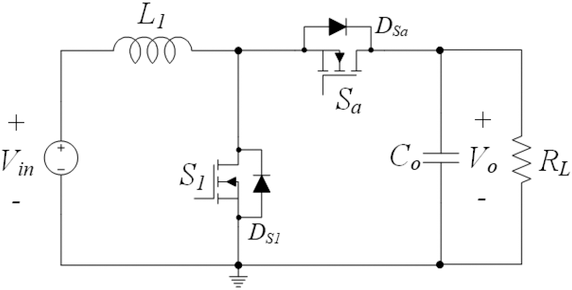
\includegraphics[width=0.5\textwidth]{Images/Implementation/Conventional-synchronous-boost-converter.png}
    \caption{Synchronous boost converter topology \cite{lee_high-efficiency_2019}.}
    \label{fig:sync_boost}
\end{figure}